\chapter{Analyse der Anwendung}\label{chapter_3}
Damit der Konfigurationsprozess für den Kunden einfacher wird, muss im ersten Schritt der aktuelle Prozess analysiert werden. Darauf aufbauend werden Konzepte zur Vereinfachung dieses Prozesses überlegt und ein neuer Workflow erstellt. Die Anforderungen an die neue Anwendung können mithilfe des neuen Prozesses anschließend spezifiziert werden.

\section{Aktueller Konfigurationsprozess}
Die Anpassungen und Vereinfachungen eines Konfigurationsprozesses bei der Verwendung von mobilen Anwendungen sollen am konkreten Anwendungsbeispiel gezeigt werden. Die Analyse beginnt bei grundlegenden Fragen, wie ein solcher Prozess aufgebaut ist und wird im Folgenden anhand eines konkreten Kundenfalls weiter ausgebaut.

\begin{figure}
\label{oldWorkflow}
\centering
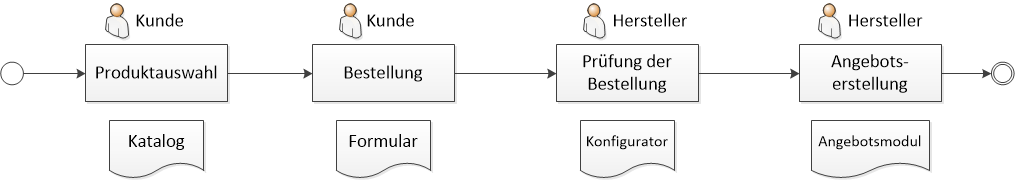
\includegraphics[width=\hsize]{images/konfigurationsprozess_alt}
\caption{Auszug eines Konfigurationsprozesses}
\end{figure}
Ein Auszug aus einem Konfigurationsprozess ist in Abbildung  \ref{oldWorkflow} zu sehen. Die Darstellung zeigt eine Vereinfachung, da in der Praxis auch Schleifen entstehen können. Zu Beginn möchte der Kunde ein konkretes Produkt auswählen. Dieses wird aus dem Katalog herausgesucht.  Anschließend kann er mithilfe von eindeutigen Produktnummern die Bestellung über ein Formular weitergeben. Damit die Zusammenstellung des Kunden geprüft werden kann, werden die Daten beim Hersteller in das Konfigurationssystem eingepflegt. Dieses berechnet die komplexen Abhängigkeiten und prüft die Gültigkeit der Konfiguration. Der letzte Schritt ist die Angebotserstellung. Hierbei wird das konkrete Angebot für den Kunden erstellt.
\par

In der Umsetzung des beschriebenen Prozesses entsteht ein Kommunikationsproblem. Dies tritt aufgrund der Trennung von Produktauswahl und der Prüfung der Bestellung durch den Produktkonfigurator auf. Der Kunde ist nur bei der Auswahl beteiligt. Das Feedback für die Umsetzung der Zusammenstellung erfolgt erst nach der Weitergabe der Bestellung. Probleme zeigen sich, wenn bei der Konfiguration Alternativen auftreten, die vom Kunden zu entscheiden sind, oder eine Konfiguration komplett nicht umsetzbar ist. Hier muss ggf. der Prozess wiederholt werden. Für die Lösung ist eine Hinzunahme des Kunden bei der Konfigurationsüberprüfung notwendig. Das Ziel, welches durch die Erstellung einer mobilen Anwendung erreicht werden soll, ist ein schnelles Feedback bei der aktuellen Auswahl. \par 

Die zweite Stelle, an der eine Verbesserung möglich ist, befindet sich bei der Eingabe der Daten für den Produktkonfigurator und der damit verbundenen Prüfung. Der Kunde hat im vorigen Schritt bereits die Daten für eine Konfiguration erfasst. Eine zweite Erfassung kann zu Fehlern oder Kommunikationsproblemen führen. Diese Probleme entstehen bei der falschen Eingabe des bestellten Produktes. Hierdurch kann der Konfigurator ein falsches Ergebnis liefern, welches zu einem inkorrekten Angebot führt. Auch in einem solchen Fall muss der Prozess wiederholt werden. Für die Verbesserung dieser Situation wird die Auswahl des Kunden direkt an den Konfigurator übermittelt. Diese Maßnahme minimiert die Fehler bei der Erfassung. \par 

Ein weiteres Problem ist die Verwendung von Produktnummern. Diese Nummern dienen einer eindeutigen Identifizierung des Produktes bei der Bestellung. In diesem Schritt kann es passieren, dass der Kunde die falsche Produktnummer auswählt, weshalb nicht das richtige Produkt bei der Angebotserstellung verwendet wird. Bei der Produktauswahl wird dieses Problem umgangen, da die Informationen nicht notwendig sind, der Kunde interessiert sich hierbei nur für das konkrete Produkt. Für die Vereinfachung des Prozesses und eine Fehlerminimierung ist eine automatische Zuordnung der korrekten Nummer im Hintergrund die Lösung. Somit wird der direkte Umgang des Kunden mit einzelnen Produktnummern vermieden und die alleinige Auswahl des Produktes steht für den Kunden im Vordergrund. Hierdurch wird der Kunde nicht mit zu vielen Produktdetails überfordert und es entsteht eine Vereinfachung des Prozesses. \par

Zusammenfassend sind drei grundlegende Probleme beim dargestellten Konfigurationsprozess festgestellt:
\begin{itemize}

		\item zusätzlicher Kommunikationsaufwand durch zu spätes Feedback,
        \item Daten werden doppelt erfasst,
        \item Produktnummern sind für den Kunden schwierig zu handhaben.
\end{itemize}
Diese drei Punkte müssen im neuen Workflow verbessert werden.

\subsection{Übertragung auf die Anwendungsdomäne Luftfahrt}
Beim Anwendungsbeispiel in der Luftfahrt erfolgt die Auswahl der Upgrades ebenfalls über einen Produktkatalog. In diesem Katalog sind die einzelnen Upgrades aufgeführt. Die Auswahl der Produkte erfolgt über eine vorhandene Weboberfläche. Diese Oberfläche ist über die Homepage des Kunden verfügbar. Der Endkunde, im Anwendungsbeispiel eine Fluggesellschaft, wählt das gewünschte Upgrade aus dem Katalog aus. Bei der Bestellung werden die Produktcodes der Auswahl verwendet. Zusätzlich müssen die Flugzeuge angegeben werden, die das Upgrade erhalten sollen. Die Identifizierung erfolgt anhand von eindeutigen Flugzeugcodes. Beide Nummern werden im nächsten Schritt von einem Produktkonfigurator erfasst, der eine Überprüfung der Konfiguration durchführt.   \par 

Beim Kunden wird die klare Trennung der Auswahl und der Überprüfung durch die Verwendung von zwei unterschiedlichen Systemen deutlich. Die Kommunikation der beiden Systeme erfolgt über die Produkt-, bzw. Flugzeugcodes. Bei der Überprüfung der Konfiguration ist der Kunde  nicht involviert. Der Experte bearbeitet die Bestellung und pflegt diese in das System ein. Die Ergebnisse werden anschließend für den Kunden aufbereitet, so dass dieser die auftretenden Alternativen verstehen und entsprechend handeln kann. Diese Besonderheit im Anwendungsbeispiel muss bei der Umstellung des Prozesses beachtet werden. \par 
\begin{figure}[H]
\centering
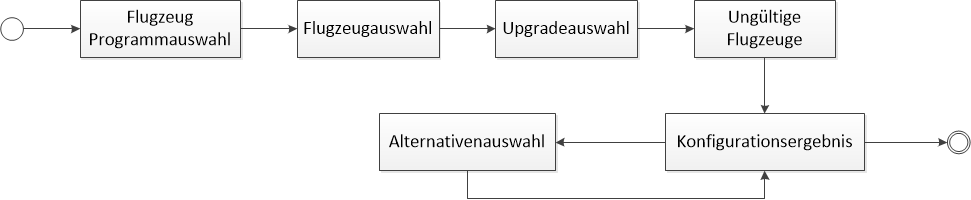
\includegraphics[width=\hsize]{images/workflow_webgui}
\caption{Programmablauf des Anwendungsbeispiels}
\label{webguiAblauf}
\end{figure}

Abbildung \ref{webguiAblauf} zeigt den Ablauf einer Konfiguration mit dem aktuellen System.
Im ersten Schritt wird das passende Flugzeugprogramm ausgewählt. Ein Programm ist eine grobe Einteilung für Flugzeuge nach deren Größe und Art. Die Auswahl ist eine erste Filterung der Datensätze. Des Weiteren werden mit Hilfe des Programms die Regeln ausgewählt, die auf dem Konfigurationsserver für eine Konfiguration verwendet werden. Anschließend folgt die Auswahl der Flugzeuge, die ein Upgrade erhalten sollen. Bei der Identifizierung für eine Bestellung wird die Flugzeugnummer angegeben. Sind die Flugzeuge ausgewählt, werden Upgrades aus einer Liste selektiert. Die Auswahl erfolgt mit der eindeutigen Nummer, welche bei der Bestellung angegeben wird. \par 

Nach dem vorigen Schritt sind alle für die Konfiguration benötigten Elemente ausgewählt. Es folgt eine Validierung der Flugzeuge. Bei dieser Überprüfung werden die einzelnen Flugzeuge auf Konfigurationen untersucht, die in einem Widerspruch mit dem ausgewählten Upgrade stehen. Wenn keine Widersprüche vorhanden sind, werden sogenannte Konfigurationsgruppen gebildet. Eine Konfigurationsgruppe enthält Flugzeuge, die in die gleichen Zielzustände kommen, wenn das Upgrade eingebaut wird. Wenn es mehrere Möglichkeiten gibt, um in einen bestimmten Zustand des Flugzeuges zu kommen, sind sogenannte Alternativen in einer Konfigurationsgruppe enthalten. Damit die Konfiguration vollständig ist, muss der Anwender für jede Gruppe eine Alternative auswählen. \par

Nachdem eine vollständige Konfiguration erzeugt wurde, wird daraus ein Excel-Dokument generiert. In diesem sind die Upgrades enthalten, die in den einzelnen Flugzeugen eingebaut werden müssen. Aus dem Dokument wird ein Upgrade-Angebot erstellt, das anschließend dem Kunden vorgelegt wird. \par 

Das Hauptproblem des aktuellen Systems ist es, dass nur Experten die Anwendung bedienen können. Eine effektive Nutzung kann nur mithilfe der Produktcodes erfolgen. Dies führt dazu, dass man ein großes Wissen über die Produktstruktur besitzen muss. Dadurch kann der Kunde die Konfiguration mit der aktuellen Anwendung nicht selbstständig durchführen. Dieses Problem wird im Folgenden bei der Modellierung des neuen Workflows gelöst.

\section{Workflow Modellierung}\label{workflow_modelling}
Der neue Workflow muss die im vorigen Abschnitt erwähnten Probleme des Konfigurationsprozesses lösen.  Anschließend müssen die Lösungen auf den konkreten Anwendungsfall übertragen werden und ein neuer Programmablauf gefunden werden.

\subsection{Umstellung auf einen mobilen Konfigurationsprozess}\label{mobileConfiguration}
Die Probleme mit der Verwendung von Produktnummern und die doppelte Erfassung der Daten lassen sich durch die Zusammenlegung von Auswahl und Konfigurationsprüfung mit einem System lösen. Diese Maßnahme ermöglicht es dem Kunden die gewünschte Auswahl zu tätigen und gleichzeitig ein Feedback der Konfiguration zu erhalten. Durch die bessere Rückmeldung verringert sich der Kommunikationsaufwand, da der Kunde im Idealfall sofort das Resultat sieht. \par 
 Für eine noch bessere Unterstützung sowie Hilfestellung beim Aufkommen von Alternativen ist die Durchführung des Prozesses mit einem Mitarbeiter des Herstellers von Vorteil. Dieser kann den Kunden durch die Konfiguration führen oder dabei unterstützen. Gleichzeitig wird hier ein besseres Verständnis für das Produkt ermöglicht. Der Hersteller hat den Vorteil einer Beschleunigung des Prozesses von der Produktauswahl bis zur Angebotserstellung. Er kann durch die direkte Auswahl der Produkte sowie ein sofortiges Prüfen und ggf. eine Selektion der Alternativen die Konfiguration abschließen und ein  Angebot erstellen. \par 
 
Diese Umstellungen des Prozesses setzt die Verwendung eines mobilen Endgerätes, in diesem Fall eines Tablet-PCs voraus. Durch die Mobilität des Gerätes kann die Konfiguration direkt beim Kunden vor Ort durchgeführt werden. Die verbesserte Kommunikationsmöglichkeit mithilfe des Tablets sorgt für ein besseres Verständnis des Kunden und dessen Wünsche. 


Zusammenfassend sind folgende zwei Maßnahmen beim neuen Workflow durchzuführen: \par

\begin{itemize}
        \item Zusammenlegen von Produktauswahl und Produktkonfiguration. 
        \item Unterstützung durch einen Mitarbeiter des Herstellers.
\end{itemize}
Die konkrete Umsetzung dieser beiden Änderungen wird im Folgenden am Anwendungsbeispiel durchgeführt. \par

\subsection{Soll-Prozess des Workflows im Anwendungsbeispiel}\label{workflowNew}
Für die Umsetzung der aus Abschnitt \ref{mobileConfiguration} erstellten Maßnahmen müssen die beiden vorhandenen Systeme für die Auswahl und Konfiguration auf ein gemeinsames Gerät portiert werden. Das Konfigurationssystem muss hierfür vereinfacht werden, um den Zugang für den Kunden zu erleichtern. Die Herausforderung besteht hier in einer übersichtlichen Darstellung der Konfigurationsergebnisse. Diese müssen für den Kunden nachvollziehbar aufbereitet werden, weil er nicht die Produktkenntnisse des Experten besitzt. Da der Kunde die Auswahl der einzelnen Produkte "'live"' vornimmt, muss die Anwendung ein schnelleres Feedback erzeugen. Bei der vorherigen Lösung hat der Experte die komplette Zusammenstellung des Kunden erhalten und musste diese in das System übertragen. Beim neuen Workflow dagegen möchte der Kunde die Reihenfolge bei der Auswahl selbst bestimmen. Dies muss im neuen Anwendungsverlauf berücksichtigt werden. \par 
\begin{figure}
\centering
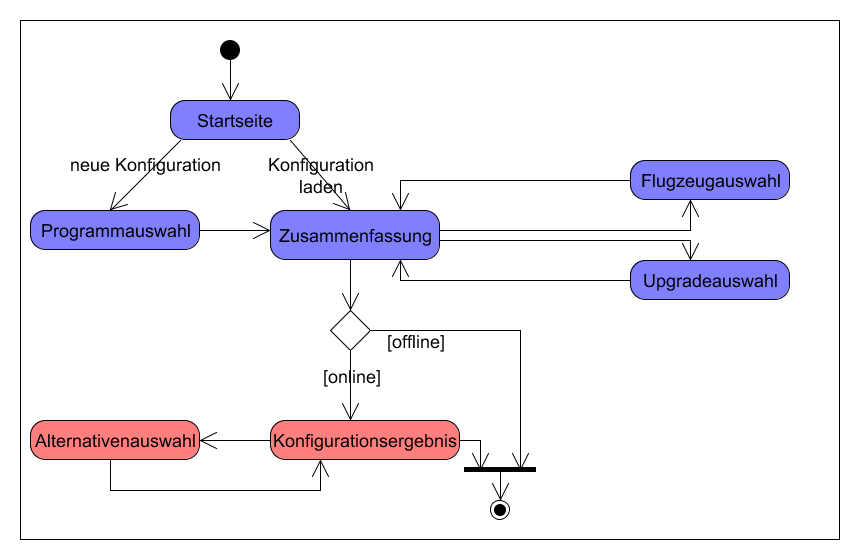
\includegraphics[width=\hsize]{images/workflow_app}
\caption{Workflow der Konfigurator-App}
\label{appWorkflow}
\end{figure}
In Abbildung \ref{appWorkflow} ist der Anwendungsverlauf der App zu sehen, welcher die benannten Problemstellen im Ist-Prozess löst. Analog zu der Weboberfläche wird bei einer neuen Konfiguration zuerst ein Programm (\textbf{Programm-auswahl}) ausgewählt. Dies ist aufgrund einer Filterung der Daten weiterhin notwendig. Nach der Auswahl gelangt der Benutzer in eine \textbf{Zusammenfassung} der aktuellen Konfiguration. Von dieser Ansicht aus können Flugzeuge (\textbf{Flugzeugauswahl}) oder  Upgrades (\textbf{Upgradeauswahl}) selektiert werden. Hier wird den unterschiedlichen Bedürfnissen des Kunden entsprochen und kein strikter Konfigurationsablauf vorgegeben, wie es im vorherigen System war. Mit dieser Umstellung wird dem Kunden die Möglichkeit gegeben die einzelnen Upgrades nacheinander zu wählen und jederzeit eine schnelle Änderung zu ermöglichen. Sobald mindestens ein Flugzeug oder ein Upgrade ausgewählt ist, wird die Konfiguration überprüft. 
Nach der Überprüfung werden die  Konfigurationsgruppen, die der Konfigurator erstellt hat, angezeigt. Diese Gruppen kann der Benutzer einsehen und bei mehreren Alternativen in einer 
separaten Ansicht (\textbf{Alternativenauswahl}) die richtige Lösung auswählen. Ist die Konfiguration vollständig, so hat der Nutzer die Möglichkeit, die aktuelle Zusammenstellung zu bestellen und den Vorgang mit der Bestellung zu beenden. 

Da die Verwendung des Konfigurationsservers, wie in Kapitel \ref{configurator} beschrieben nach dem Client-Server Modell aufgebaut ist, wird eine andere Möglichkeit bei der Konfiguration nötig. Beim mobilen Einsatz der Anwendung kann es passieren, dass eine Verbindung mit dem Konfigurationsserver nicht möglich ist. Aus diesem Grund muss es einen alternativen Weg des Workflows geben. Wenn der Konfigurationsserver nicht verfügbar ist, wird die Konfiguration gespeichert, damit eine Prüfung später durchgeführt werden kann. In diesem Fall ist der Prozesses mit der Speicherung der Konfiguration beendet.

\subsection{Prozessbeteiligte der Anwendung}
Nach der Umstellung des Konfigurationsprozesses müssen die Benutzer der Anwendung identifiziert werden. Dies ist eine Voraussetzung, um die Anforderungen für die Zielgruppe passend zu definieren. Der neue Prozess ist darauf ausgelegt, dass ein Vertreter des Flugzeugherstellers zusammen mit einem Endkunden die Konfiguration durchführt. Der Kunde im Anwendungsbeispiel ist kein unerfahrener Laie. Stattdessen ist er für Upgrades der vorhandenen Flugzeugflotte einer Fluggesellschaft zuständig. Somit ist bereits ein Wissen über das Produkt vorhanden. Dies hat zur Folge, dass der Kunde die Struktur und den Aufbau des Flugzeuges kennt. Dadurch unterscheidet sich die Konfiguration bspw. zu einem Online-Konfigurator eines Autoherstellers. Hier sind unerfahrene Anwender die Zielgruppe, denen der Aufbau des Produktes auf eine andere Weise erklärt werden müsste. \par 
\begin{figure}
\centering
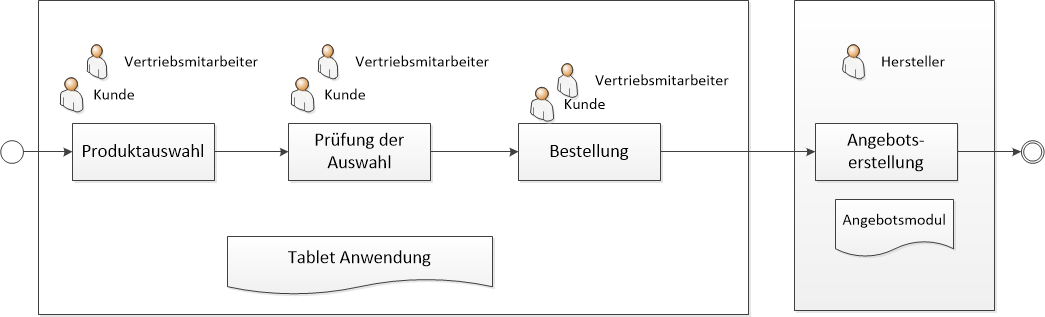
\includegraphics[width=\hsize]{images/konfigurationsprozess_neu}
\caption{Anwendungsbereiche der Tablet Anwendung}
\label{newWorkflow}
\end{figure}
Betrachtet man die Zielgruppe im Workflow des Anwendungsbeispiels,  so stellt man fest, dass
zuvor die Produktauswahl sowie die Bestellung dem Kunden überlassen wurde. Die neue Tablet Anwendung vereint die einzelnen Prozessschritte, so dass am Ende eine direkte Bestellung folgen kann, die zu einem Angebot führt. Die Durchführung des Konfigurationsprozesses wird im Zusammenwirken von Kunde und Anbieter durchgeführt (siehe Abbildung \ref{newWorkflow}). Dies hat zur Folge, dass die App für zwei unterschiedliche Zielgruppen konzipiert werden muss.


\section{Anforderungsanalyse} \label{requirements}
Nachdem der grundlegende Prozess auf die Bedürfnisse des Kunden sowie an die mobile Umgebung angepasst ist, können daraus die Anforderungen der Anwendung für das Anwendungsbeispiel festgelegt werden. Bei der Festlegung wird zuerst die allgemeine Anforderung erläutert sowie anschließend auf das Anwendungsbeispiel spezifiziert. Zur übersichtlichen Darstellung wird im Folgenden zwischen funktionalen und nicht-funktionalen Anforderungen unterschieden. 

\subsection{Nicht-Funktionale Anforderungen}\label{non_functional_requirements}
Die nicht-funktionalen Anforderungen betreffen alle Maßnahmen zur Vereinfachung, bzw. Unterstützung des Prozesses sowie Anforderungen aufgrund des vorhandenen Systems. Diese speziellen Voraussetzungen sind für den Benutzer meistens nicht sichtbar und laufen im Hintergrund, bzw. unbewusst ab. Aus diesem Grund müssen hier auch spezielle Gütekriterien festgelegt werden, um am Ende eine Evaluation dieser nicht-funktionalen Anforderungen zu ermöglichen. Als Basis werden die 10 Heuristiken für Benutzerschnittstellen von Nielsen \cite{bib:heuristicsNielsen} verwendet.
Analog lassen sich aus dem neuen Workflow folgende Anforderungen spezifizieren:


\paragraph{Einfache Bedienung:} Der Kunde ist kein Experte und verwendet die Anwendung nicht jeden Tag somit ist eine einfache Bedienung eine Voraussetzung. Je weniger bei der Verwendung der Software erklärt werden muss, desto besser ist diese Anforderung erfüllt. Für die Erfüllung dieses Ziels sollen folgende Schwerpunkte der Softwareergonomie \cite{bib:softwareErgonomie} beachtet werden: 
\begin{itemize}
        \item Selbstbeschreibungsfähigkeit,
        \item Lernförderlichkeit,
        \item Erwartungskonformität.
\end{itemize}
Die Kriterien nach Nielsen sind Konsistenz, Erkennung vor Erinnerung und Sichtbarkeit des Systemstatus.

\paragraph{Schnelle Bedienung:} Die zweite Zielgruppe der Anwendung ist der Experte. Für diesen muss es die Möglichkeit einer schnellen Bedienung der Anwendung geben, sodass er die Konfiguration möglichst effizient gestalten kann. Somit wird eine flexible Bedienung der Anwendung nötig. Für eine zusätzliche Steigerung der Effizienz muss die Navigation zwischen den einzelnen Seiten schnell sein. Dies bedeutet, dass beim Übergang von einer zur nächsten Seite der Benutzer nicht lange warten sollte. Ebenfalls muss es genügend Feedback geben, wenn ein Seitenwechsel länger dauern sollte. Hier werden die beiden Heuristiken Sichtbarkeit des aktuellen Status und Flexibilität sowie Effizienz bei der Benutzung beachtet.

\paragraph{Optimierung auf die Umgebung: } Da ein mobiles Gerät nur begrenzte oder eingeschränkte Resourcen zur Verfügung hat, müssen die einzelnen Bedienelemente auf die Umgebung angepasst sein. Ebenfalls muss die Bedienung für eine Touch-Eingabe optimiert sein. 
Für ein einheitliches Aussehen der Anwendung müssen die Richtlinien der jeweiligen Technologie beachtet werden. Diese Anforderung enthält die beiden Heuristiken ästhetisches und minimalistisches Design sowie Standards und Konsistenz.

Für eine bessere Übersicht der nicht-funktionalen Anforderungen sind diese in der Tabelle \ref{nonFunctionalRequ} dargestellt. Zu jeder Anforderung wird hier ein zusätzlicher Bezeichner definiert.

\begin{table}
\begin{tabular}{| p{0.7cm} | p{2.2cm} | p{4.5cm} | p{5.5cm}|}
\toprule[2pt] \rowcolor{dunkelgrau}
\hline
  Bez. & Anforderung & Beschreibung & Heuristiken nach Nielson \\
  \hline
  N1 & Einfache \newline Bedienung & Die Anwendung soll von unerfahrenen Benutzern bedient werden können.& \begin{itemize}
          \item Sichtbarkeit des aktuellen Status
          \item Erkennung vor Erinnerung
          \item Sichtbarkeit des aktuellen Status
  \end{itemize} \\
  \hline
  N2 & Schnelle \newline Bedienung & Experten müssen die Anwendung schnell und effizient bedienen können. & \begin{itemize}
            \item Flexibilität und Effizienz bei Benutzung
            \item Sichtbarkeit des aktuellen Status
    \end{itemize}  \\
  \hline
    N3 & Optimierung auf Umgebung & Die Anwendung muss auf die Zielplattform optimiert werden. &  \begin{itemize}
              \item Ästhetisches und minimalistisches Design
              \item Standards und Konsistenz
      \end{itemize} \\
    \hline
\bottomrule[2pt]
\end{tabular}
\caption{Nicht-Funktionale Anforderungen mit Bezeichner}
\label{nonFunctionalRequ}
\end{table}

\subsection{Funktionale Anforderungen}\label{functionRequ}
Die funktionalen Anforderungen sind von der Prozessbeschreibung im Abschnitt \ref{mobileConfiguration} abhängig. Im Folgenden werden diese speziell auf das Anwendungsprojekt spezifiziert. Zusätzlich zu der Spezifikation wird der Bezug zum neuen Workflow hergestellt:

\paragraph{Filterung der Anwendungsdaten: } Da sehr viele Daten vorhanden sind, müssen diese für eine übersichtliche Darstellung im Vorfeld gefiltert werden. Die Filterung erfolgt in zwei Schritten:
\begin{enumerate}
\item Auswahl der Kundendaten: Die Anwendung soll speziell bei einem Kunden eingesetzt werden. Aus diesem Grund kommen nur die kundenspezifischen Daten zum Einsatz.
\item Programmauswahl: Durch die Wahl des Programmes wird eine Filterung der einzelnen Flugzeuge und der möglichen Updates erreicht.
\end{enumerate}
Diese Anforderung wird ebenfalls durch die Verwendung einer mobilen Umgebung notwendig. Damit der zweite modellierte Workflow mit einer nicht vorhandenen Internetverbindung funktioniert, müssen die Daten offline verfügbar sein. Da nur begrenzte Speichermöglichkeiten auf dem Gerät vorhanden sind, können nicht alle Kundendaten gespeichert werden. Dies bedingt eine Filterung durch die Auswahl des Kunden.

\paragraph{Upgradeauswahl: } Bei der Auswahl von Upgrades im Anwendungsbeispiel werden die Funktionen des Produktkataloges benötigt. Es muss möglich sein, ein bestimmtes Produkt an- oder abzuwählen. Damit der Kunde den Aufbau des Produktes versteht, müssen die einzelnen Produkte nach einer bestimmten Struktur geordnet sein. 

\paragraph{Flugzeugauswahl: } Flugzeuge, die ein ausgewähltes Upgrade erhalten sollen, müssen ebenfalls in der Anwendung auswählbar sein. Die Anforderungen an diese Auswahl sind nicht die Gleichen wie bei der Produktauswahl. Der Schwerpunkt muss hier auf ein schnelles Finden der einzelnen Flugzeuge gelegt werden. Dies wird ebenfalls durch eine dem Kunden bekannte Struktur erreicht. 

\paragraph{Anzeige der Konfigurationsergebnisse: } Damit der Kunde ein schnelles Feedback der aktuellen Auswahl erhält, müssen die Konfigurationsergebnisse angezeigt werden. Dies impliziert eine Anbindung an den Konfigurationsserver, der die entsprechenden Ergebnisse berechnet. Diese Anzeige muss eine vereinfachte Darstellung beinhalten, damit der Kunde diese Ergebnisse verstehen kann.

\paragraph{Alternativenauswahl: } Damit eine vollständige Konfiguration erzeugt werden kann, muss die Anwendung eine Auswahl für Alternativen bereitstellen. Hierbei muss das Verständnis des Kunden für das Produkt berücksichtigt werden. Die Alternativen müssen auf eine verständliche Art dargestellt sein. 

\paragraph{Speichern und Laden der Konfiguration: } Die zweite Voraussetzung des alternativen Offline Workflows ist eine Speicherung der Konfiguration. Für eine spätere Bearbeitung ist das erneute Laden der Konfiguration notwendig. Diese beide Anforderungen werden aufgrund der mobilen Zielumgebung benötigt.

Die Zuordnung der einzelnen Anforderungen zu den jeweiligen Prozessschritten ist in Tabelle \ref{functionalRequirements} zu sehen. Hierbei werden die drei Prozessanforderungen Produktkatalog, Konfiguration und mobile Zielumgebung unterschieden.
\par 
\begin{table}

\begin{tabular}[H]{| p{0.4cm} | p{2.5cm} | p{5.9cm} | p{4.5cm} |}
\toprule[2pt] \rowcolor{dunkelgrau}
\hline
  NR. & Anforderung & Beschreibung & Prozesszuordnung \\
  \hline
  F1 & Upgrade-auswahl & Es sollen Upgrades für Flugzeuge auswählbar sein & Produktkatalog
   \\
  \hline
  F2 & Flugzeug-auswahl & Es müssen Flugzeuge eines bestimmten Kunden auswählbar sein. & Produktkatalog  \\
  \hline
    F3 & Konfigurations-ergebnisse anzeigen & Übersichtliche Darstellung der aktuellen Zusammenstellung & Konfiguration \\
    \hline
     F4 & Alternativen-auswahl & Bei mehreren Möglichkeiten einer Auswahl sollen Alternativen ausgewählt werden können & Konfiguration \\
        \hline
    F5 & Speichern und Laden & Die getätigte Auswahl soll gespeichert und geladen werden können& mobile Zielumgebung \\
    \hline
    F6 & Filterung der Anwendungsdaten & Die Daten (Flugzeuge und Upgrades) müssen gefiltert werden können & mobile Zielumgebung \\
    \hline
\bottomrule[2pt]
\end{tabular}
\caption{Funktionale Anforderungen mit Bezeichner}
\label{functionalRequirements}
\end{table}





